\documentclass[a4paper,12pt]{article}
\usepackage{tikz}
\usetikzlibrary{calc}
\begin{document}

\begin{figure}
\centering
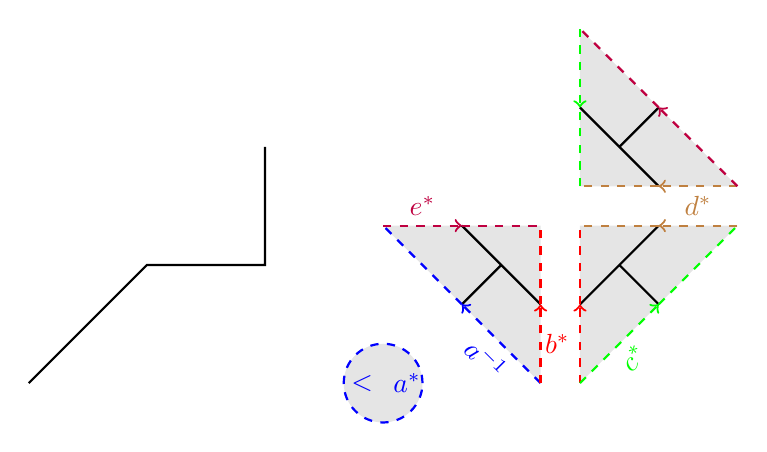
\begin{tikzpicture}[line width=0.8pt,scale=0.5]
\foreach \i in {-9,...,9}{
	\foreach \j in {-9,...,9}{
		\coordinate(v\i\j) at (\i,\j);
		\foreach \k in {0,...,9}{
			\coordinate(v\i\j\k) at ($(v\i\j)+(\k*36-18: 0.4)$);
		}
	}
}

%% Cercle elliptique
\fill [gray!20] (v00) circle (1);
\draw [blue, dashed] (v00) circle (1);

\draw [blue] (v00) node[left]{$<$} node[right]{$a^*$};


%% triangle bas gauche

\fill [gray!20] (v40)--(v04)--(v44)--cycle;
\draw (v22)--(v33)--(v42)--(v33)--(v24);

%a*^-1
\draw [blue,dashed ,->](v40)--(v22)node[midway,sloped, below]{$a^{-1}$};
\draw [blue, dashed](v22)--(v04);

% b*^{-1}
\draw [red, dashed,->](v40)--(v42);
\draw [red, dashed](v42)--(v44);

%e^*
\draw [purple,dashed, ->] (v04)--(v24)node[midway, above]{$e^*$};
\draw [purple,dashed ] (v24)--(v44);

%% triangle bas droite

\fill [gray!20] (v54)--(v94)--(v50)--cycle;
\draw (v63)--(v72)--(v63)--(v52)--(v63)--(v74);

%b^*
\draw [red, dashed, ->] (v50)--(v52)node[midway, left]{$b^*$};
\draw [red, dashed] (v52)--(v54);

%c^*
\draw [green, dashed,->] (v50)--(v72)node[midway, sloped, below]{$c^*$};
\draw [green, dashed] (v72)--(v94);

%d^*
\draw [brown, dashed,->] (v94)--(v74)node[midway, above]{$d^*$};
\draw [brown, dashed] (v74)--(v54);

%% triangle haut droite
\fill [gray!20] (v55)--(v59)--(v95)--cycle;
\draw (v57)--(v75)--(v66)--(v77);

%d*^-1
\draw [brown, dashed, ->] (v95)--(v75);
\draw [brown, dashed] (v75)--(v55);

%c*^-1
\draw [green, dashed] (v55)--(v57);
\draw [green, dashed, ->] (v59)--(v57);

\draw [purple, dashed,->] (v95)--(v77);
\draw [purple, dashed] (v77)--(v59);



\draw (v-90)--(v-63)--(v-33)--(v-36);
%e c^-1 e^-1 c^-1

%\draw (v20)--(v31)--(v51)--(v53);
%\draw (2,0)--(4/3+2,4/3)--(8/3+2,4/3)--(8/3+2,8/3);
%\draw (8/3+2,4/3)--(10/3+2,2/3);

\end{tikzpicture}
\end{figure}

\begin{figure}
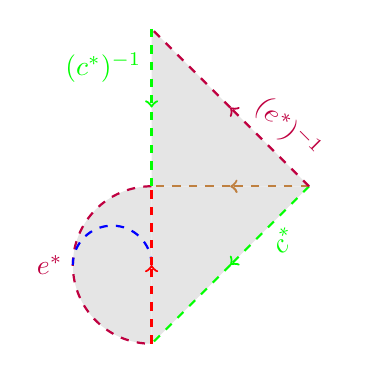
\begin{tikzpicture}[line width=0.8pt,scale=0.5]
\foreach \i in {-9,...,9}{
	\foreach \j in {-9,...,9}{
		\coordinate(v\i\j) at (\i,\j);
		\foreach \k in {0,...,9}{
			\coordinate(v\i\j\k) at ($(v\i\j)+(\k*36-18: 0.4)$);
		}
	}
}

%% Cercle e
\fill [gray!20] (v04) arc (90:270:2);
\draw [purple, dashed] (v04) arc (90:270:2) node[midway,left]{$e^*$};

\draw [blue, dashed] (v02) arc (0:180:1);



%% triangle bas droite

\fill [gray!20] (v44)--(v04)--(v00)--cycle;

%b^*
\draw [red, dashed, ->] (v00)--(v02);
\draw [red, dashed] (v02)--(v04);

%c^*
\draw [green, dashed,->] (v44)--(v22)node[midway, sloped, below]{$c^*$};
\draw [green, dashed] (v22)--(v00);

%d^*
\draw [brown, dashed,->] (v44)--(v24);
\draw [brown, dashed] (v24)--(v04);

%% triangle haut droite
\fill [gray!20] (v04)--(v08)--(v44)--cycle;
%d*^-1
\draw [brown, dashed, ->] (v44)--(v24);
\draw [brown, dashed] (v24)--(v04);

%c*^-1
\draw [green, dashed] (v04)--(v06);
\draw [green, dashed, ->] (v08)--(v06)node[midway, left]{$(c^*)^{-1}$};

\draw [purple, dashed,->] (v44)--(v26)node[midway, sloped, above]{$(e^*)^{-1}$};
\draw [purple, dashed] (v26)--(v08);

\end{tikzpicture}
\end{figure}
\begin{figure}
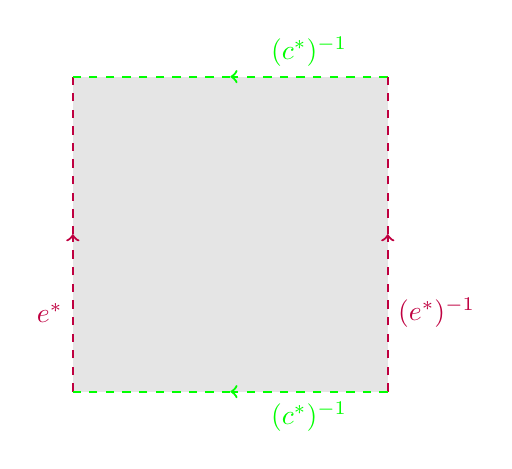
\begin{tikzpicture}[line width=0.8pt,scale=0.5]
\foreach \i in {-9,...,9}{
	\foreach \j in {-9,...,9}{
		\coordinate(v\i\j) at (\i,\j);
		\foreach \k in {0,...,9}{
			\coordinate(v\i\j\k) at ($(v\i\j)+(\k*36-18: 0.4)$);
		}
	}
}
% Torus
\fill [gray!20] (v00)--(v08)--(v88)--(v80)--cycle;
%e*
\draw [purple, dashed,->] (v00)--(v04)node[midway,left]{$e^*$};
\draw [purple, dashed] (v04)--(v08);

%c*^-1
\draw [green, dashed,->] (v88)--(v48)node[midway,above]{$(c^*)^{-1}$};
\draw [green, dashed] (v48)--(v08);

%e*^-1
\draw [purple, dashed,->] (v80)--(v84)node[midway,right]{$(e^*)^{-1}$};
\draw [purple, dashed] (v84)--(v88);

%c*
\draw [green, dashed,->] (v80)--(v40)node[midway,below]{$(c^*)^{-1}$};
\draw [green, dashed] (v40)--(v00);
\end{tikzpicture}
\end{figure}
\end{document}



